\documentclass[a4paper,10pt]{article}

\usepackage[italian]{babel}
\usepackage[utf8]{inputenc}

\usepackage{amsfonts}
\usepackage[inline]{asymptote}
\usepackage[backend=biber]{biblatex}
\usepackage{caption}
\usepackage{csquotes}
\usepackage{geometry}
\usepackage{graphicx}
\usepackage{minted}

\addbibresource{references.bib}

\title{Train Radar \\ Documentazione tecnica}
\author{Bortolin Alessandro, 5BIA}
\date{8 febbraio 2020}

\begin{document}
\maketitle

\begin{abstract}
  \emph{Train Radar} è l'applicazione che ti permette di seguire in tempo reale i treni in tutta Italia! Questa applicazione si ispira a \emph{flighradar24} \cite{flighradar}, un'applicazione che mostra la posizione degli aerei in tutto il mondo in diretta, tuttavia non esiste alcuna applicazione simile sul Play Store per i treni. Grazie a \emph{Train Radar} puoi monitorare i treni di qualsiasi regione, ordinarli in base alla propria distanza e monitorare i ritardi di ogni treno!
\end{abstract}

\section{Dettagli tecnici}

  \subsection{Activity}
    L'applicazione possiede tre activity con cui l'utente può interagire:

    \medskip
    \noindent
    \texttt{RadarActivity} è l'activity principale, mostra all'utente la mappa con la posizione dei treni e permette di cercare un treno specifico.

    \medskip
    \noindent
    \texttt{TrainActivity} mostra le informazioni principali del treno selezionato con la lista delle fermate e la mappa del tragitto.

    \medskip
    \noindent
    \texttt{NearTrainsActivity} mostra una lista con tutti i treni ordinati per distanza.

  \subsection{Fragment}
    \medskip
    \noindent
    \texttt{TrainDetailFragment} viene mostrato all'interno della \texttt{RadarActivity} quando l'utente interagisce con un treno, mostra le informazioni principali del treno.

    \medskip
    \noindent
    \texttt{TrainRouteFragment} si trova dentro il \texttt{ViewPager} all'interno della \texttt{TrainActivity}, mostra le informazioni principali di un treno ed il suo tragitto.

    \medskip
    \noindent
    \texttt{TrainMapFragment}, come il \texttt{TrainRouteFragment}, si trova dentro il \texttt{ViewPager} all'interno della \texttt{TrainActivity} attraverso un \texttt{ViewPager}, mostra la mappa con il tragitto del treno.

  \subsection{MapView}
    L'applicazione possiede una \texttt{MapView} \cite{mapssdk} per mostrare la mappa dei treni limitata al territorio italiano.

  \subsection{Intent}
    L'applicazione possiede un \texttt{Intent} per passare dalla \texttt{RadarActivity} alla \texttt{NearTrainsActivity} in cui viene passata la posizione. Inoltre sia la \texttt{RadarActivity} che la \texttt{NearTrainsActivity} possiedono un \texttt{Intent} per avviare la \texttt{TrainActivity} in cui vengono passate le informazioni relative al treno selezionato. Agli \texttt{Intent}, se possibile, vengono passate informazioni ausiliarie in modo da animare la transizione tra le activity al meglio \cite{sharedelements}.

  \subsection{Handler}
    La posizione di ogni treno mostrato nell'activity principale viene aggiornata in tempo reale. Questa operazione viene eseguita mediante un \texttt{Handler} in modo da programmare la sua esecuzione ad un intervallo regolare di un secondo.

  \subsection{AsyncTask}
    Calcolare la posizione dei treni è un'operazione relativamente pesante e richiede approssimativamente 100ms. Per dare un'interfaccia fluida all'utente tale operazione viene eseguita in background mediante un \texttt{AsyncTask}.

  \subsection{Internet}
    L'applicazione necessita di una connessione ad internet in modo da visualizzare la mappa con i treni e aggiornare in tempo reale il ritardo dei treni \cite{tiapi}.

  \subsection{Geolocalizzazione}
    L'utente può anche acconsentire all'applicazione di usare i dati relativi alla propria posizione geografica, in tal modo l'utente può visualizzare i treni nelle proprie vicinanze riordinati per distanza.

  \subsection{Supporto per schermi orizzontali}
    L'applicazione supporta sia lo schermo in modalità verticale sia in modalità orizzontali \cite{compatibility}. Le activity sono state ottimizzate in modo da supportare al meglio l'orientamento dello schermo.

    \medskip
    \noindent
    Nell'activity \texttt{RadarActivity} la descrizione del treno selezionato viene mostrata in basso quando lo schermo è verticale mentre viene mostrata di lato quando lo schermo è orizzontale.

    \medskip
    \noindent
    Nell'activity \texttt{TrainActivity} viene mostrato un layout scrollabile con due pagine in modalità verticale, mentre in modalità orizzontale vengono mostrate entrambe le pagine (figure \ref{port} e \ref{land}).

    \begin{figure}[h!]
      \begin{minipage}{0.45\textwidth}
        \centering
        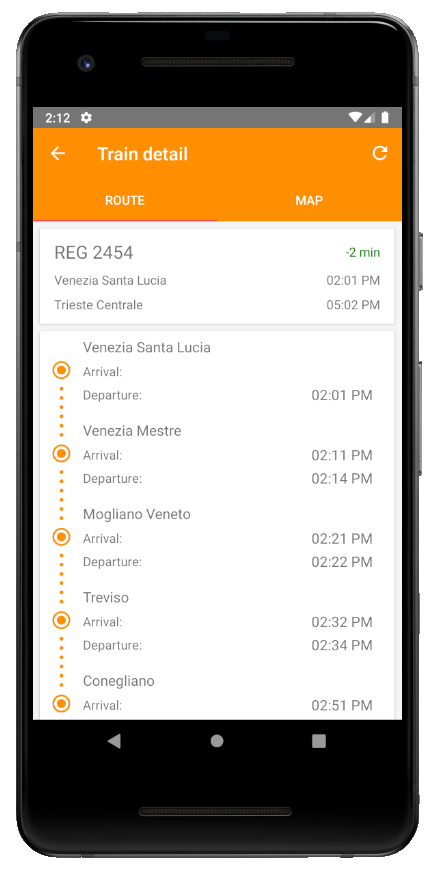
\includegraphics[width=0.4\textwidth]{images/port}
        \captionsetup{justification=centering}
        \caption{Schermo in modalità verticale}
        \label{port}
      \end{minipage}
      \hfill
      \begin{minipage}{0.50\textwidth}
        \centering
        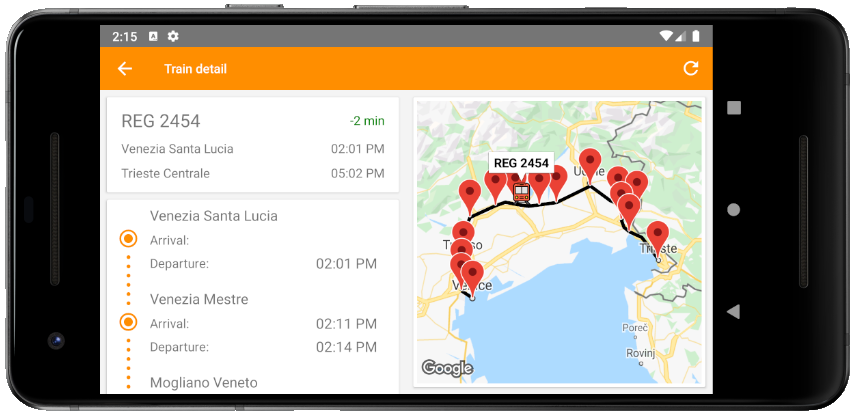
\includegraphics[width=0.7\textwidth]{images/land}
        \captionsetup{justification=centering}
        \caption{Schermo in modalità orizzontale}
        \label{land}
      \end{minipage}
    \end{figure}

    \medskip
    \noindent
    Nell'activity \texttt{NearTrainsActivity} in modalità orizzontale la lista dei treni viene visualizzata con due colonne anziché una sola.

  \subsection{Librerie di terze parti}
    La libreria \emph{Gson} \cite{gson} è stata utilizzata per serializzare e deserializzare i dati in formato json.

    \medskip
    \noindent
    La libreria \emph{Volley} \cite{volley} è stata utilizzata per eseguire le richieste HTTP delle API di \emph{Trenitalia}.

\section{Caratteristiche principali}
  La caratteristica principale dell'applicazione è la possibilità di monitorare in tempo reale la posizione dei treni in tutta Italia, questo aspetto contraddistingue \emph{Train Radar} da tutte le altre applicazioni presenti nel Play Store. L'applicazione inoltre fornisce i ritardi di ogni treno in modo da garantire affidabilità agli utenti. Un'altra caratteristica importante è la versatilità poiché l'applicazione mira ad un pubblico vasto e non necessita di particolari conoscenza per utilizzarla, inoltre per garantire al meglio la versatilità l'applicazione supporta in modo completo sia la visualizzazione in verticale che in orizzontale. \emph{Train Radar} necessita di una connessione ad internet per poter funzionare tuttavia l'applicazione dispone di una cache per ridurre al minimo tale consumo e poter utilizzarla in qualsiasi situazione.

\section{Struttura dell'applicazione}
  L'applicazione è molto semplice ed intuitiva, nell'activity principale è presente una mappa con cui l'utente può interagire, muovendosi e visualizzando i treni nella zona selezionata, clickando sopra di un treno l'utente può visualizzare le informazioni relative a tale treno. Nella barra superiore dell'activity è presente un menù con cui l'utente può spostarsi alle altre activity. Se l'utente acconsente a fornire le informazioni relative alla propria posizione, nella mappa verrà mostrato un marcatore a segnalarla e clickando tale marcatore si aprirà un'activity mostrante la lista di tutti i treni presenti ordinati per distanza assoluta. Clickando a sua volta un treno della lista si aprirà un'ulteriore activity contenente tutte le informazione del treno ed una mappa con il suo tragitto. Quest'ultima activity è anche accessibile dall'activity principale interagendo con un determinato treno.

  \begin{figure}[h!]
    \centering
    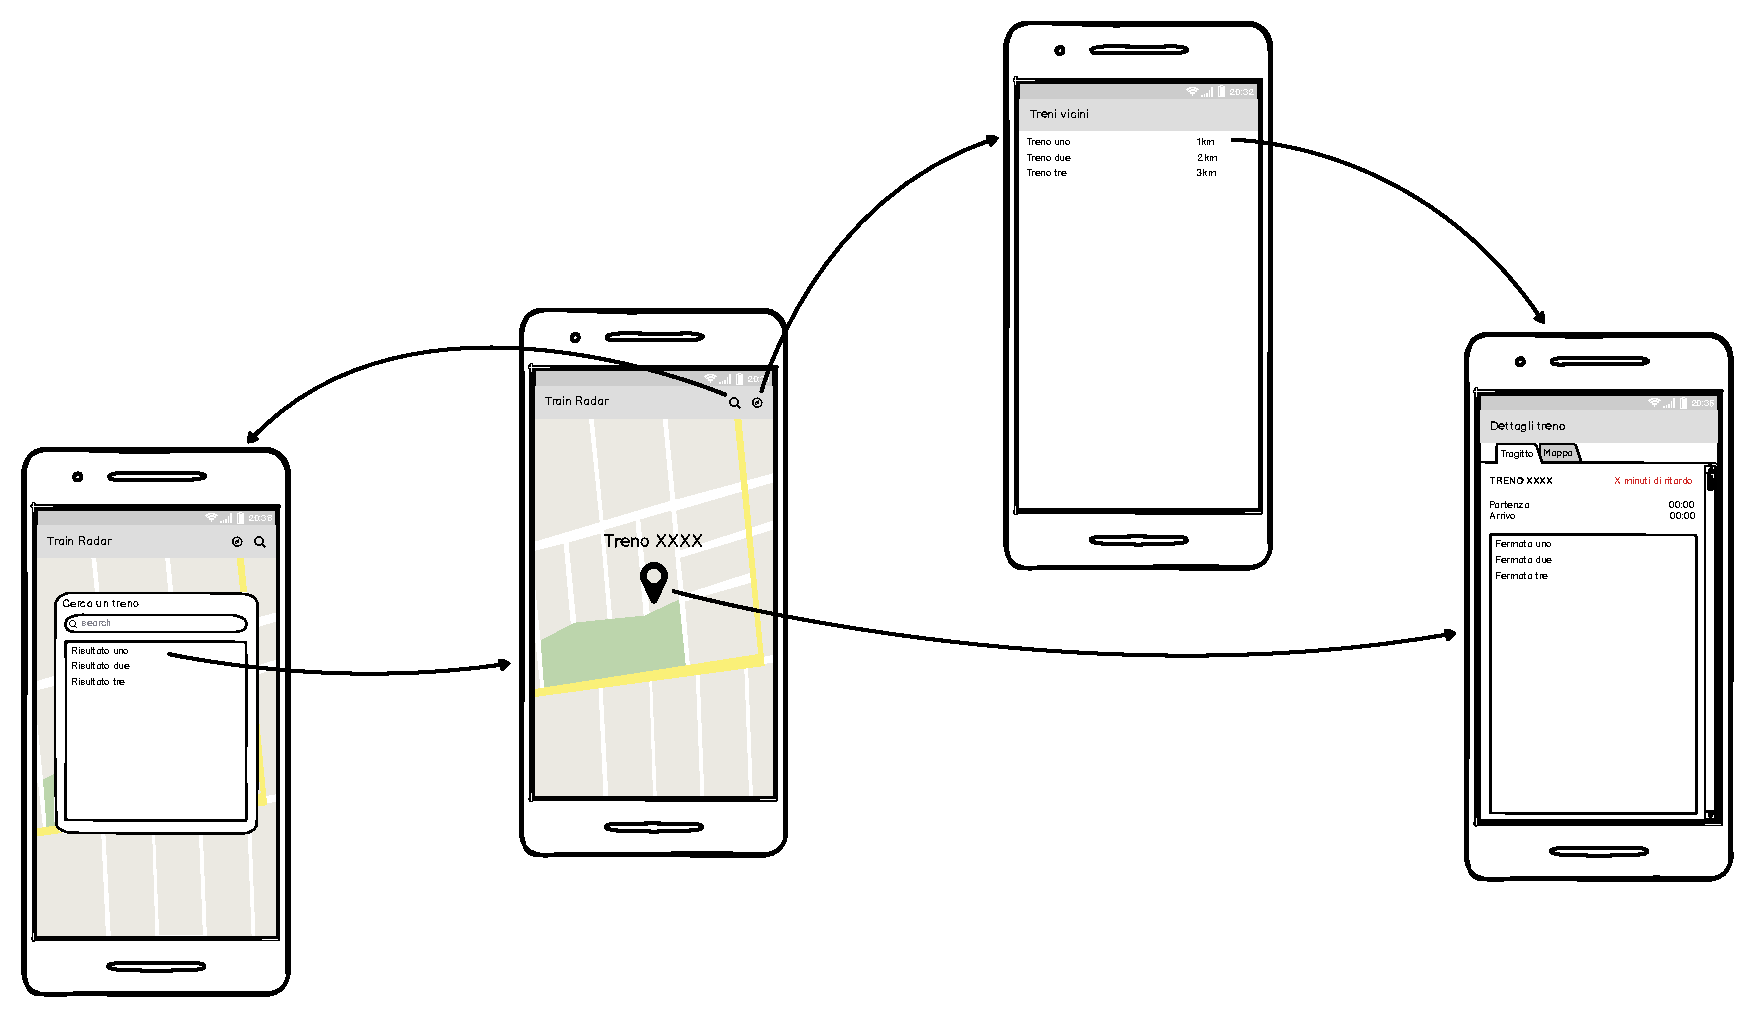
\includegraphics[width=0.9\textwidth]{images/wireframe}
    \caption{Wireframe dell'applicazione}
  \end{figure}

  \begin{figure}[h!]
    \centering
    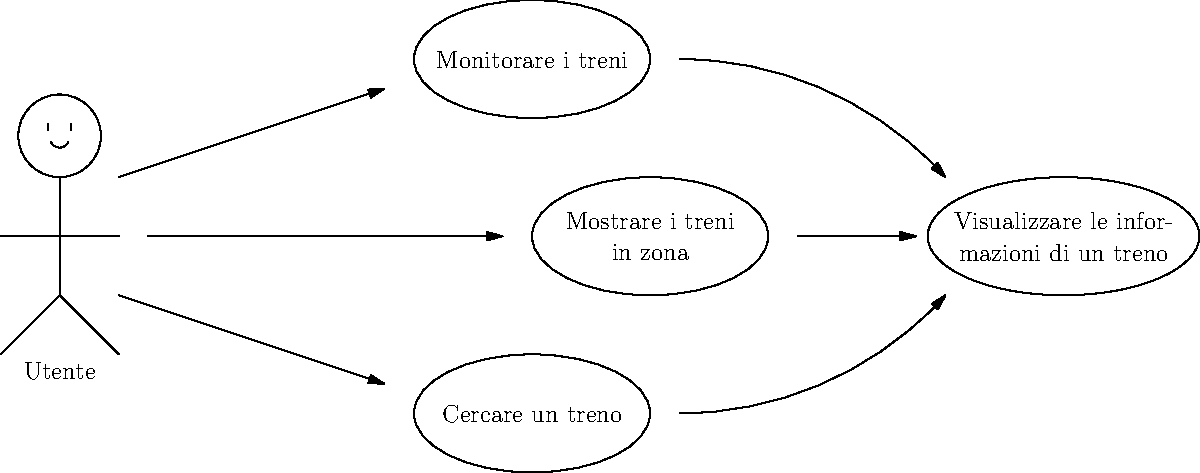
\includegraphics[width=0.9\textwidth]{asy/use_case_diagram}
    \caption{Diagramma d'uso dell'applicazione}
  \end{figure}

\pagebreak

\section{Frammenti di codice}
  Il cuore dell'applicazione sono le classi base che rappresentano i treni e le stazioni, esse contengono le informazioni principali di ogni treno e stazione.

  \medskip
  \begin{minipage}[t]{0.45\textwidth}
    \inputminted{java}{snippet/Train.java}
  \end{minipage}
  \hfill
  \begin{minipage}[t]{0.45\textwidth}
    \inputminted{java}{snippet/Station.java}
  \end{minipage}

  \medskip
  \noindent
  Ad ogni treno mostrato nella mappa viene associato un \texttt{Marker} in cui viene sostituita l'icona di default con una rappresentante un treno.
  \inputminted{java}{snippet/Marker.java}

  \medskip
  \noindent
  Per aggiornare la posizione di treno viene usato un \texttt{Handler} che ricalcola la posizione del treno ogni secondo.
  \inputminted{java}{snippet/Scheduler.java}

  \medskip
  \noindent
  Per calcolare la posizione di un treno tra due stazioni si usa l'algoritmo di Dijkstra in modo da trovare il percorso atteso meglio approssimato.
  \inputminted[fontsize=\footnotesize]{java}{snippet/Dijkstra.java}

\section{Sviluppo}
  \parbox{4cm}{Target API level:}    29 \\
  \parbox{4cm}{Minimum API level:}   26 \\
  \parbox{4cm}{IDE:}                 Android Studio

  \subsection{Difficoltà riscontrate}
    \paragraph{Calcolo della posizione dei treni}
      \emph{Trenitalia} non fornisce direttamente la posizione dei treni, perciò è stato richiesto un \emph{workaround} per ottenerla. Per prima cosa, grazie alle API di \emph{Trenitalia} \cite{tiapi} si possono ricavare le coordinate geografiche della maggior parte delle stazione, successivamente si può calcolare un'approssimazione della posizione calcolando la posizione attesa in linea d'aria tra l'ultima stazione visitata e la successiva stazione. Tuttavia questa tecnica fallisca con treni a lunga tratta (ad esempio Milano-Roma senza fermate intermedie), per migliorare ulteriormente la posizione si può rappresentare le ferrovie italiane come un grafo ed utilizzare l'algoritmo di Dijkstra \cite{dijkstra} per ottenere un percorso più preciso.

    \paragraph{Gestione dei thread}
      La posizione dei treni viene calcolata in background in modo da lasciare fluida l'esperienza dell'utente, tuttavia ciò ha richiesto un ulteriore sforzo per sincronizzare i thread. Il principale problema avveniva quando si cambiava activity mentre stava avvenendo un aggiornamento della posizione causando un crash dell'applicazione. Il problema è stato risolto mediante i monitor del Java.

    \paragraph{Transizioni delle activity}
      Nelle transizioni tra due activity vengono visualizzate delle animazioni \cite{sharedelements} dove alcuni elementi comuni alle due activity vengono mantenuti, tuttavia ciò non funzionava nella activity \texttt{TrainActivity} poiché utilizzando un \texttt{ViewPager} il contenuto dell'activity veniva visualizzato attraverso un \texttt{Fragment} che veniva processato leggermente più tardi rispetto alla creazione dell'activity. Il problema è stato risolto utilizzando \texttt{postponeEnterTransition()} e \texttt{startPostponedEnterTransition()}.

  \subsection{Bug noti}
    \paragraph{Tratte non aggiornate}
      \emph{Train Radar} salva tutte le tratte in un database locale, tuttavia dato che \emph{Trenitalia} cambia frequentemente gli orari delle proprie tratte, può capitare che un treno in realtà cancellato venga comunque mostrato e viceversa un treno in programma non venga mostrato. Purtroppo l'unico modo per correggere questo bug è aggiornare quotidianamente tutte le tratte che però è un'operazione lunga e pesante e non fattibile in pratica.

    \paragraph{Ritardo dei treni}
      Per rendere il consumo di dati più leggero, \emph{Train Radar} calcola il ritardo solo dei treno mostrati nella mappa. Questo implica che se un treno è già arrivato in programma, ma in realtà ha accumulato un ritardo e perciò è ancora in viaggio, \emph{Train Radar} supponendo che sia già arrivato non calcola il ritardo di tale treno e perciò non lo mostra nella mappa.

  \subsection{Sviluppi futuri}
    Per adesso \emph{Train Radar} mostra la posizione dei treni solo di \emph{Trenitalia} e di \emph{Trenord}, tuttavia in Italia ci sono decine di altre imprese ferroviare come ad esempio \emph{Italo}. L'applicazione può essere migliorata aggiungendo il supporto a queste società ferroviarie.

  \subsection{Autovalutazione}
    Nel complesso darei un voto di 4.5 su 5 all'applicazione poiché è molto utile, ben strutturata, semplice e si rivolge verso un pubblico di molto vasto. Chiunque con la passione dei treni apprezzerebbe questa applicazione.

\medskip

\printbibliography

\end{document}
